\chapter{Background Materials}
\label{chap:chbg}

This chapter provides the mathematical background on OT and kernel methods, with concepts that are most relevant to this thesis. 

We assume familiarity with basic measure-theoretic concepts \citep{rudin}.
We recall that the notations $\calX, \ \calY$ denote the subspaces where the support of the two given measures lie. This thesis considers the setting when $\calX$ and $\calY$ are comparable spaces \footnote{For an extension of OT to incomparable spaces, we refer the readers to the Gromov Wasserstein variant detailed in \cite{tvayer-thesis}.}. Further, for the simplicity of notations, we take $\calX=\calY=\R^d$ $(d>0)$. 
\section{Background on Optimal Transport (OT)}\label{bg:ot}
In the late 1700s, the French mathematician Gaspard Monge posed the question of finding a measurable function, $T$, to ``optimally" transform a distribution $s_0\in \calR_1^+(\calX)$ to $t_0\in \calR_1^+(\calX)$. Here, the optimality is quantified based on a pre-specified cost function $c~:~\calX\times \calX \mapsto \R$ over the support. 

The \textbf{Monge-OT} problem \citep{monge} between distributions $s_0,\ t_0\in \calR_1^+(\calX)$ can be expressed as the following optimization problem: 
\begin{equation}\label{monge-ot}
\inf\left\{ \int c\left(x, T(x)\right)\ \textup{d}s_0(x)~:~T_{\#}s_0=t_0 \right\},
\end{equation}
where $T_{\#}s_0=t_0$ denotes the mass-preservation constraints, mathematically expanded as $s_0(x\in T^{-1}(A))=s_0(T(x)\in A)=t_0(x\in A)$ for all Borel sets $A\subseteq \calX$. This is pictorially illustrated in Fig. \ref{fig:mass-pres} when $\calX=\R$. The distribution $s_0$ is referred to as the \textit{source distribution} and the distribution $t_0$ as the \textit{target distribution}. The \textit{optimal value} of this problem gives a divergence between distributions $s_0$ and $t_0$, and the \textit{optimal solution} to this problem, called the Monge-OT map, provides a mapping between the two support sets.
\begin{figure}[ht]
    \centering
    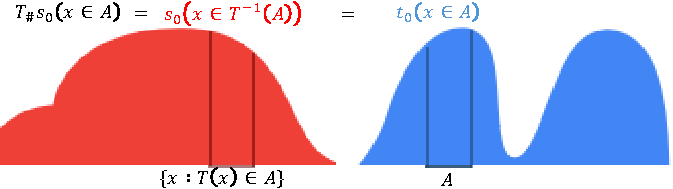
\includegraphics[scale=0.8]{background/images/mass-pres.pdf}
    \caption[Illustration of the mass-preservation constraints in Monge-OT.]{Illustration of the mass-preservation constraints in Monge-OT with $A$ as an arbitrary Borel measurable subset of the support and $T$ as the transformation function from $s_0$ to $t_0$.}\label{fig:mass-pres}
\end{figure}

This formulation established the mathematical foundations for geometry-induced divergences between measures that \textit{lift} the geometry (captured through the ground metric, $c$) over their support. However, the non-linear feasibility set in the Monge-OT optimization problem (Eq.~\ref{monge-ot}) prompts several questions about the existence and uniqueness of the solution to this optimization problem. \cite{brenier} studied settings where the Monge-OT attains a unique solution, for example, when the cost function is squared-Euclidean $c(x, y)=\|x-y\|^2$. While such characterizations make the Monge-OT theory more rigorous, there are also cases where the solution set of Monge-OT is empty. Consider a simple example when $\calX=\R$ and the discrete distributions $s_0=\delta_{x_0}$ and $t_0 = \frac{1}{2}(\delta_{x_1}+\delta_{x_2})$, $x_0\neq x_1\neq x_2$. One can not construct a function $T$ that satisfies the mass-preservation constraints. It is easy to see this by ruling out different possibilities, i.e. the function $T(x_0)=x_i$ for $i\in \{1, 2\}$ results in $s_0(x_0)\neq t_0(T(x_0))$, thus violating the constraints.

In the above example, one may want a solution that transports half the mass from $x_0$ to $x_1$ and half the mass from $x_0$ to $x_2$. Such solutions can be obtained through a relaxed variant of the Monge-OT problem proposed by \cite{KatoroOT}. Kantorovich-OT re-formulates the OT problem to optimize for a \textit{probabilistic transport coupling} over the distributions.
\subsection{On Kantorovich-OT}\label{bg:ot-variants}
Given a cost function, $c:\calX\times\calX\mapsto\R$, and two probability measures $s_0\in\calR^+_1(\calX),\ t_0\in\calR^+_1(\calX)$, the $p$-Wasserstein Kantorovich-OT ($p\geq 1$) formulation is defined as follows.
\begin{definition}[$p$-Wasserstein Kantorovich-OT; $p\geq 1$]
\begin{equation}\label{eqn:kot}
\bar{W}_{c, p}^p(s_0,t_0)\coloneqq \min\limits_{\pi\in\calR^+_1(\calX\times\calX)}\int c^p\ \textup{d}\pi, \textup{ s.t.}\ \ \pi_1=s_0,\ \pi_2=t_0.
\end{equation}
\end{definition}
The notations $\pi_1$ and $\pi_2$ denote the first and the second marginals of the transport coupling $\pi$ obtained as $\pi(\cdot,\  \calX)$ and $\pi(\calX, \ \cdot)$, respectively. The constraints are, therefore, referred to as the marginal-matching constraints or the mass-preservation constraints.

An \textit{optimal solution} to the Kantorovich-OT problem  (Problem~\ref{eqn:kot}) is called an optimal coupling or an optimal transport plan (OT plan).
Whenever the cost is a valid distance metric, over $\calX\times \calX$, called the ground metric, the \textit{optimal value} gives the $p$-Wasserstein metric, over $\calR^+_1(\calX) \times \calR^+_1(\calX)$. This metricity is concluded based on the following three properties satisfied by $\bar{W}_{c, p}(s_0,\ t_0)$: 
\begin{itemize}
    \item Non-negativity: $\bar{W}_{c, p}(s_0,\ t_0)\geq 0$; $\bar{W}_{c, p}(s_0,\ t_0)= 0 \iff s_0=t_0$
    \item Symmetry: $\bar{W}_{c, p}(s_0,\ t_0)=\bar{W}_{c, p}(t_0,\ s_0)$
    \item Triangle-inequality: $\bar{W}_{c, p}(s_0,\ t_0)\leq \bar{W}_{c, p}(s_0,\ u_0) + \bar{W}_{c, p}(u_0,\ t_0)$, for any $u_0\in \calR_1^+(\calX)$.
\end{itemize}
%In particular, $\bar{W}_1$ is a metric belonging to the family of Integral Probability Metrics and is the same as the Kantorovich metric.
The cost metric over the supports is also called as the \textit{ground metric}.
Unlike the case of the Monge-OT problem (\ref{monge-ot}), the solution to the Kantorovich-OT problem always exists as there is always a feasible coupling characterized by $\pi(A\times B)=s_0(A)\cdot t_0(B)$ for any Borel sets $A, B\subseteq \calX$.

A popular approach to deriving an OT map from an OT plan is through the Barycentric-Projection problem: $T(x)\equiv \argmin_{y\in \calX} \E_{Y\sim \pi(\cdot|X=x)}[c(y, Y)|X=x],$
where the conditional $\pi(\cdot|X=x)
$ is computed from the OT plan solution of the Kantorovich-OT problem. The Barycentric-Projection has a closed-form solution in some special cases, like when the cost function is squared-Euclidean, $T(x)=\E_{\pi(\cdot|X=x)}[Y|X=x]$.
\stoptoc
\subsubsection{Dual Formulation}
Under mild assumptions, the Kantorovich-OT formulation admits strong duality \citep[Theorem (1.42)]{santab}, which we discuss below.
\begin{definition}[Dual of Kantorovich OT]
Whenever $c$ is lower semi-continuous and bounded from below, then the duality result of the Kantorovich-OT problem (\ref{eqn:kot}) gives the following.
\begin{align}
    \bar{W}_{c, p}^p(s_0, t_0) &= \max\limits_{f\in\calC(\calX),g\in\calC(\calX)}\int_\calX f\ \textup{d}s_0+\int_\calX g\ \textup{d}t_0, \nonumber\\
    &\ \textup{s.t.}\ f(x)+g(y)\le c^p(x,y)\ \forall\ x,y\in\calX.
\end{align}
\end{definition}
The functions $f$ and $g$ are called Kantorovich potential functions.
\noindent
A famous duality result is that of Kantorovich-Rubinstein for 1-Wasserstein.
\begin{align*}
    \bar{W}_{c, 1}(s_0, t_0) = &\max\limits_{f\in \calW_c} \int_\calX f\ \textup{d}s_0-\int_\calX f\ \textup{d}t_0,\nonumber\\
    &\textup{where }\calW_c\equiv \left\{ f:\calX\mapsto \mathbb{R} :~ \max\limits_{x\in\calX\neq y\in\calX} \frac{|f(x)-f(y)|}{c(x, y)} \leq 1 \right\}.
\end{align*}
The RHS is also known as the Kantorovich metric, which belongs to the family of Integral Probability Metrics (IPMs) \citep{Sriperumbudur09onintegral}. Unlike the Wasserstein metric, the Kantorovich metric is well-defined even for unnormalized measures that may have unequal masses.

\subsubsection{Wasserstein Barycenter}
The geometry induced by a metric can be studied by characterizing its interpolation properties. The $p$-Wasserstein barycenter between $s_0, t_0\in \calR^+_1(\calX)$, interpolating according to the weight $\rho\in [0, 1]$, is obtained as the solution to $
    \min\limits_{u_0\in \calR^+_1(\calX)} \rho\bar{W}_{c, p}(s_0, u_0)  + (1-\rho)\bar{W}_{c, p}(u_0, t_0).$
For the case of 1-Wasserstein, the solution to the problem is simply $\rho s_0 + (1-\rho)t_0$ (the empirical average). More popularly, the Wasserstein barycenter is computed with the divergence $\bar{W}_{c, 2}^2 $, with $c$ as squared-Euclidean, which doesn't have an analytical form in general.

\subsubsection{$f$-Divergence-regularized OT}
The applicability of Kantorovich-OT formulation is limited to normalized probability measures, which is the reason Kantorovich-OT is also called Balanced OT. In particular, when the source and target measures have different masses, one can not find a transport plan whose marginals' masses exactly match the masses of the source and target measures. Furthermore, in applications where one only has access to empirical measures, which could be noisy, one may not want to enforce these mass-preservation constraints exactly. To cater to such settings, the Unbalanced OT (UOT) formulation was introduced, which we will detail below.


Given a cost function, $c:\calX\times\calX\mapsto\R$, and measures, $s_0\in \calR^+(\calX)$ and $t_0\in \calR^+(\calX)$, the unbalanced optimal transport approach~\citep{Liero2018,chizat17,chizat18a} learns a transport plan that incurs the least expected cost, enforcing regularization-based soft constraints for mass-preservation. KL-divergence and, in general, $f$-divergence (\citep{Csiszar67},~\citep{Sriperumbudur09onintegral}) based regularizations have been popularly studied in the UOT setting. 
\begin{definition}[$f$-Divergence-regularized OT]
The $f$-divergence regularized OT formulation \citep[Eq. (2.4)]{chizat17} is given as:
\begin{equation}\label{bgeqn:uot}
\min\limits_{\pi\in\calR^+\left(\calX\times\calX\right)}\ \int c\ \textup{d}\pi + \lambda D_f(\pi_1,s_0) + \lambda D_f(\pi_2,t_0),
\end{equation}
where $D_f(\cdot,\cdot)$ denotes the $f$-divergence (\citep{Csiszar67,Sriperumbudur09onintegral}) between two measures.
\end{definition}

UOT with KL-divergence-based regularization (KL-OT) induces the so-called Gaussian Hellinger-Kantorovich metric~\citep{Liero2018} between the measures whenever $0<\lambda\leq 1$ and the ground cost $c$ is the squared-Euclidean distance.

UOT with TV-divergence-based regularization (TV-OT) induces the so-called Generalized Wasserstein metric~\citep{Piccoli2014GeneralizedWD} between the measures whenever $\lambda>0$ and the ground cost $c$ is a valid metric.
\resumetoc
\subsection{Computational Aspects}\label{bg:comp}
\stoptoc
\subsubsection{Closed-form Solutions}
There are special cases where the closed-form solution of the Kantorovich-OT (\ref{eqn:kot}) problem is known. 

\noindent Let $s_0, t_0\in \calR_1^+(\R)$ have cumulative distribution functions, $F^{s_0}$ and $F^{t_0}$, respectively. Then, if the cost function $c(x, y) = |x-y|$, we have the following.
\begin{align}\nonumber
    \bar{W}^p_{c, p}(s_0, t_0) = \int_0^1 \left| \left(F^{s_0}\right)^{\dagger}(t) - \left(F^{t_0}\right)^{\dagger}(t) \right|^p \textup{d}t,
\end{align}
where $\left(F^{s_0}\right)^{\dagger}(x)\equiv \inf\{t: \ F^{s_0}(t)\geq x\}$.
A general version of this result, along with the proof, can be found in \citet[Proposition (2.17)]{santab}. This closed-form computation of Wasserstein lays the foundation for Sliced-Wasserstein variants \citep{bonet2023leveraging} that alleviate the curse of dimensionality issue by solving for one-dimensional projections of the involved measures.

A more popular setup where the OT problem has a closed-form solution is that with Gaussian measures over $\R^d$ and the cost function being squared-Euclidean:
$$\bar{W}_{c, 2}^2\left(\mathcal{N}(\mathbf{m_1}, \bm{\Sigma}_1),\ \mathcal{N}(\mathbf{m_2}, \bm{\Sigma}_2)\right) = \|\mathbf{m_1}-\mathbf{m_2}\|^2 + \mathcal{B}^2(\bm{\Sigma}_1, \bm{\Sigma}_2),$$ where $\mathcal{B}(\bm{\Sigma}_1, \bm{\Sigma}_2)\coloneqq \sqrt{\rm{Tr}\left(\bm{\Sigma}_1+\bm{\Sigma}_2-2\left(\bm{\Sigma}^{1/2}_1\bm{\Sigma}_2\bm{\Sigma}^{1/2}_1\right)^{1/2} \right)}$ is called the Bures metric.
Moreover, the OT map has the form $T: x\mapsto \mathbf{m}_2+ \mathbf{A}(x-\mathbf{m}_1)$, where $\mathbf{A}=\bm{\Sigma}_1^{-1/2}\left(\bm{\Sigma}_1^{1/2}\bm{\Sigma}_2\bm{\Sigma}_1^{1/2} \right)^{1/2}\bm{\Sigma}_1^{-1/2}$.
A derivation of this result can be found in \citet[Example (1.19)]{Chewi2024StatisticalOT}.
Similarly, in this setup, the resulting Wasserstein barycenter with interpolation weight $\rho\in [0, 1]$ is again a Gaussian, with mean $\mathbf{m}=\rho \mathbf{m}_1+(1-\rho)\mathbf{m}_2$ and the covariance as the solution to the problem $\min\limits_{\bm{\Sigma}\succcurlyeq 0}\rho \calB^2(\bm{\Sigma}_1, \bm{\Sigma})+(1-\rho)\calB^2(\bm{\Sigma}, \bm{\Sigma}_2)$ \citep[Remark (9.5)]{peyre2019computational}.

There are also useful bounds that relate the Wasserstein distance between (arbitrary) non-Gaussian measures to that between Gaussian measures.
Let $s', t'\in \calR_1^+(\calX)$ have the same moments up to order two as the Gaussian distributions $s_0, t_0\in \calR_1^+(\calX)$. Then \cite{lbWass} show that $\bar{W}_{c, 2}(s_0, t_0)\geq \bar{W}_{c, 2}(s', t')$.

\subsubsection{Finite-Sample-based Estimators} In the preceding discussion, we saw a few cases where Kantorovich-OT obtained a closed-form solution. However, in general, solving the Kantorovich-OT problem (\ref{eqn:kot}) involves solving an optimization problem.
While the Kantorovich-OT optimizes over all non-negative densities (the set, $\calR_1^+(\calX\times \calX)$), implementing this in practice is often not feasible. Also, in typical ML applications, we only have access to discrete empirical measures rather than the true measures. Consider the empirical/discrete measures\footnote{Equal number of samples taken for the simplicity of notations.} $\hat{s}_m=\sum_{i=1}^m (\mathbf{s}_m)_i\delta_{x_{1i}}$ and $\hat{t}_m=\sum_{j=1}^m (\mathbf{t}_m)_j\delta_{x_{2j}}$, where $\mathbf{s}_m, \mathbf{t}_m\in \mathbb{R}_+^m$ and $\mathbf{s}_m^\top \bone_m = \mathbf{t}_m^\top \bone_m=1$. Here, a pragmatic choice for learning the transport plan is to learn a finitely-parameterized matrix, $\bgamma \in \mathbb{R}_+^{m\times m}$, supported over the empirical samples, with $\bgamma_{ij}$ denoting the probability of coupling the samples $x_{1i}$ and $x_{2j}$ from the two distributions (Fig.~\ref{discOT}).

In this practical setting, we discuss the simplifications of Kantorovich-OT formulation as follows.
\begin{definition}[Finite-Sample-based Kantorovich-OT]
\begin{equation}\label{eqn:discretekot}
\widehat{W}^p_{c, p, m}(\hat{s}_m,\hat{t}_m)\coloneqq \min\limits_{\bgamma\in \Delta_{m^2}}\Tr(\bgamma \bC^\top), \textup{ s.t.}\ \ \bgamma \bone_m=\mathbf{s}_m,\ \bgamma^\top \bone_m=\mathbf{t}_n,
\end{equation}
where $\Delta_{m^2}$ denotes an $(m^2-1)$-dimensional simplex, $\bC\in \R^{m\times m}$ is the cost matrix with $\bC_{ij}=c^p(x_{1i}, x_{2j})$ and $\Tr(\cdot)$ denotes the trace of the specified matrix.
\end{definition}
\begin{figure}[t]
    \centering
    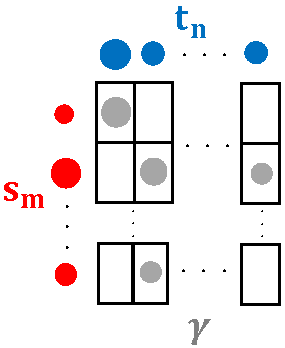
\includegraphics[scale=0.5]{background/images/discOT.pdf}
    \caption[Illustration of an optimal coupling or an OT plan (solution of Kantorovich-OT) in the discrete setting.]{Illustration of an optimal coupling or an OT plan (solution of Kantorovich-OT, $\bgamma$) in the discrete setting. The blobs represent the amount of probability mass values at different support points.}
    \label{discOT}
\end{figure}

This finite-sample-based OT formulation allows the applicability of standard solvers. To approximate the original Kantorovich-OT problem (\ref{eqn:kot}) with Problem \ref{discOT}, one would want to have as many samples ($m$) as possible. However, one can see that with increasing $m$, the memory requirements in Problem \ref{discOT} to store $\bC$ and $\bgamma$ also scale quadratically.
 A popular approach to alleviate this issue is to solve the OT problem over smaller subsets (mini-batches) and then perform an aggregation. Recent statistical guarantees in \cite{fatras2019learnwass,jumbot} have backed the applicability of this minibatch-OT approach.

\subsubsection{Entropy-regularized OT}\label{entOT} Problem \ref{discOT} has the constraint set $\Gamma\equiv \{ \bgamma: \bgamma \in \Delta_{m^2}; \ \bgamma \bone_n = \mathbf{s}_m;\ \bgamma^\top \bone_m = \mathbf{t}_n \}$ which is a convex set and the objective $\rm{Tr}(\bgamma\bC^\top)=\langle \bgamma, \bC \rangle$ is a linear function in $\bgamma$. Thus, we can see that $\widehat{W}^p_{c, p, m}$ can be solved with standard solvers for Linear Programs. However, the resulting computation of $O(m^3)$ \citep{peyre2019computational} is a bottleneck for large-scale ML applications. \cite{cuturi13a} proposed the Kantorovich-OT problem with an additional entropic regularization on the OT plan and showed scalable Sinkhorn-algorithm-based solvers.
\begin{definition}[Entropy-regularized OT \citep{cuturi13a}]
\begin{equation}\label{entropyOT}
    \hat{E}_{c,\epsilon}(\hat{s}_m, \hat{t}_n)\coloneqq \min\limits_{\bgamma\in \Gamma} \rm{Tr}(\bgamma\bC^\top) - \epsilon H(\bgamma),
\end{equation}
where $H(\bgamma)$ denotes the Shannon entropy $\sum_{i, j}\bgamma_{ij}\log{\frac{1}{\bgamma_{ij}}}$.   
\end{definition}
The function $(\hat{s}_m, \hat{t}_n) \mapsto \mathbbm{1}_{\hat{s}_m\neq \hat{t}_n} \hat{E}_{c,\epsilon}(\hat{s}_m, \hat{t}_n)$ satisfies all properties of a metric whenever $c$ is a metric.
The entropy-regularized OT problem becomes differentiable with a strictly convex objective that implies it admits a unique minimizer. The main advantage of the entropy-regularized OT formulation is computational efficiency, which is discussed next.

We present a few details for solving Problem \ref{entropyOT}, which is a Convex Program, and hence, one can alternatively solve its dual program. With Lagrangian variables as $\mathbf{u}\in \R^m$ and $\mathbf{v}\in \R^n$ for the marginal constraints, the first order conditions for the optimization $\min_{\bgamma> \bzero} \ \Tr(\bgamma\bC^\top)-\epsilon H(\bgamma)-\langle \mathbf{u}, \bgamma\bone_n-\mathbf{s}_m \rangle - \langle \mathbf{v}, \bgamma^\top \bone_m - \mathbf{t}_n \rangle$ leads to the solution $\bgamma=\textup{diag}(\bar{\mathbf{u}})\mathbf{M}\textup{diag}(\bar{\mathbf{v}})$, where $\bar{\mathbf{u}}_i= e^{\mathbf{u}_i/\epsilon}$, $\bar{\mathbf{v}}_j= e^{\mathbf{v}_j/\epsilon}$ and $\mathbf{M}=\exp{\left(-\frac{\bC}{\epsilon}\right)}$. Here, $\textup{diag}(\cdot)$ represents a matrix with the diagonal entries as the entries of the argument vector.
Now, the Sinkhorn algorithm to find $\bar{\mathbf{u}}$ and $\bar{\mathbf{v}}$ utilizes the marginal-constraints satisfaction criteria. Starting with initial vectors $\bar{\mathbf{u}}^0$ and $\bar{\mathbf{v}}^0$, the updates at iteration $t$ are done as $\bar{\mathbf{u}}^{t}\coloneqq \frac{\mathbf{s}_m}{\mathbf{M}\bar{\mathbf{v}}^{t-1}}$ and $\bar{\mathbf{v}}^{t}\coloneqq \frac{\mathbf{t}_n}{\mathbf{M}^\top\bar{\mathbf{u}}^{t}}$. Each iteration requires a computation cost of $O(mn)$. These matrix-vector products are highly parallelizable operations on a GPU, which leads to the computational efficiency of the entropic OT formulation. 
Such entropy-regularized formulations have also helped scale the computation of Wasserstein barycenters and the UOT formulation with KL-divergence \citep{ChizatPSV18}.
% \cite{Sinkhorn}
\resumetoc
\subsection{Statistical Aspects}\label{bg:ot-stats}
Statistical OT involves studying the rates at which the Wasserstein metrics estimated from empirical samples converge to the true Wasserstein metrics. The following theorem shows the issue of the curse of dimensionality, due to which one may need an exponential number of samples to estimate the metric in higher dimensions.
\begin{theorem}[Proposition 1 in \cite{nilesweed2019estimation}] Let $s_0\in \calR_1^+([-1, 1]^d)$. Let $\hat{s}_m$ be an empirical measure over $m$ IID samples from $s_0$, then for any $p\in [1, \infty)$,
    $\E[\bar{W}_{c, p}(\hat{s}_m, s_0)]\leq O(m^{-\frac{1}{d}})$ if $d>2p$.
\end{theorem}


% \begin{theorem}[Restated from \cite{dudley1969}] With distributions $s_0,\ t_0 \in \calR_1^+(\R^d)$ ($d>2$) having bounded support, we have the following statistical convergence result for $p$-Wasserstein ($p>1$):
% $$\E\left[ \left| \bar{W}_{c, p}(\hat{s}_m, \hat{t}_m) - \bar{W}_{c, p}(s_0, t_0)  \right| \right] = O\left( m^{-1/d} \right). $$
% \end{theorem}
Here, the expectation is over the randomness in the empirical samples. With the use of triangle inequality, the estimation rate $\bar{W}_{c, p}(s_0, t_0)\leq O(m^{-\frac{1}{d}})$. Further, a lower bound can be established by considering uniform measures over $[-1, 1]^d$. \cite{nilesweed2019estimation} presented an improved bound for the special case when the distributions satisfy the spiked transport model \citep[Eq. (2)]{nilesweed2019estimation}. However, this improved bound still has an adversarial dependence on $d$. Such results bottleneck the usage of Kantorovich-OT in high-dimensional ML applications. A detailed review of such statistical aspects can be found in \cite{Chewi2024StatisticalOT}. Our work tries to alleviate such issues by incorporating concepts from kernel methods, which are discussed in the next section.
\newline
\newline
\textit{With this, we conclude our discussion on the mathematical background of OT that is the most relevant to this thesis.
We refer the readers to \cite{peyre2019computational} for details on other variants of the Kantorovich-OT problem. For the readers interested in diving deeper into the theoretical aspects of OT, we refer to \cite{villanioldnew,santab} and \cite{Chewi2024StatisticalOT}.}
\section{Background on Kernel Methods}
%Let $\calX$ denote the subspace  
A Hilbert space is a vector space with an inner product that is complete (i.e. all Cauchy sequences converge). Analogous to the concept of inner products in Euclidean spaces, kernels are used to compute the inner product in a Hilbert space of functions. In the subsequent sections, we discuss kernel functions and the computational as well as statistical aspects of kernel methods.
\subsection{On Kernels and the MMD Metric}\label{bg:kme}
\stoptoc
\subsubsection{Kernel Function} A function $k: \calX\times \calX \mapsto \R$ is called a positive definite kernel function if it is a symmetric function i.e. $k(x, y) = k(y, x)\ \forall x, y\in \calX$ and $\sum_{i,j=1}^m \mathbf{a}_i\mathbf{a}_j k(x_i, x_j) \geq 0$ for any $m\in \mathbb{N}$, any $x_1, \cdots, x_m \in \calX$ and any $\mathbf{a}\in \R^m$. The last condition can be expressed as the positive semi-definiteness of a matrix containing the kernel function evaluations. Such a matrix is called the \textit{Gram matrix}, $\bG\in \R^{m\times m}$, with $\bG_{ij}=k(x_i, x_j), \ i, j\in [m]$. 

\begin{theorem}[Reproducing Kernel Hilbert Space. Restated from \cite{mohri2018foundations}]
    Let $k:\calX\times \calX\mapsto \R$ be a positive definite kernel. Then, there exists a Hilbert Space $\calH_k$ and a feature map $\phi_k:\calX \mapsto \calH_k$ such that $k(x, y) = \langle \phi_k(x), \phi_k(y) \rangle \ \forall x, y\in \calX$.
    \newline
    Furthermore, $\calH_k$ satisfies the \textit{reproducing property} given as $ f(x) = \langle f, k(x, \cdot) \rangle \ \forall x\in \calX,\ f\in \calH_k$.
    \newline
    This Hilbert space $\calH_k$ is called a reproducing kernel Hilbert space (RKHS) associated with $k$. $\|\cdot\|_k$ is the norm induced by the inner product in $\calH_k$: $\|f\|_k=\sqrt{\langle f, f \rangle}\ \forall f\in \calH_k$.
\end{theorem}
The original theorem, along with the proof, can be found in \citet[Theorem (6.8)]{mohri2018foundations}. Below, we give an example of a kernel and the associated feature map.

%We present the following example that originally appeared as Example 16.2 in \cite{Mohri}.
\begin{example}[Gaussian Kernel over $\R\times \R$]
Consider the mapping $\phi_k$ such that for each $n\in \mathbb{N}$, $\left(\phi_k(x)\right)_n = \frac{1}{n!}e^{-\frac{x^2}{2\sigma^2}}x^n$, $x\in \R$. Then, 
\begin{align*}
    \langle\phi_k(x), \phi_k(y)\rangle &= \sum_{n=0}^\infty \left(\frac{1}{n!}e^{-\frac{x^2}{2\sigma^2}}x^n\right)\cdot \left(\frac{1}{n!}e^{-\frac{y^2}{2\sigma^2}}y^n\right)\\
    &=e^{-\frac{\|x-y\|^2}{2\sigma^2}} \tag{Gaussian/RBF kernel.}
\end{align*}
\end{example}
A positive-definite kernel $k$ on $\calX$ is called \textit{normalized} if $k(x,x)=1,\ \forall x \in \calX$. As $k(x, x)=\langle \phi_k(x), \phi_k(x) \rangle=\|\phi_k(x)\|_k^2$, for a normalized kernel $k$, $\|\phi_k(x)\|_k=1\ \forall x\in \calX$. A normalized positive definite kernel $k':\calX\times \calX \mapsto \R$ can be obtained from any positive-definite kernel $k$ by defining $k'(x, y) = \begin{cases}
0 & \textup{if }\left(k(x, x)\cdot k(y, y)=0\right)\\
\frac{k(x, y)}{\sqrt{k(x, x)k(y, y)}} & \textup{otherwise}.
\end{cases}$ $ \forall x, y\in \calX$.
A positive-definite kernel $k$ on $\calX$ is called \textit{bounded} if $|k(x, y)|<\infty,\ \forall x,\ y\in \calX$.
A continuous positive-definite kernel $k$ on $\calX$ is called \textit{c-universal} if the RKHS $\calH_k$ is dense in $\calC(\calX)$ w.r.t. the sup-norm, i.e., for every function $g \in \calC(\calX)$ and all $\epsilon>0$, there exists an $f\in\calH_k$ such that $\|f-g\|_\infty\leq \epsilon$. Gaussian kernel (RBF kernel) is an example of a universal kernel over the continuous domain. Dirac delta kernel, $k(x, y)=1_{x\neq y}$, is an example of a universal kernel over the discrete domain.

\subsubsection{Maximum Mean Discrepancy (MMD)} This section discusses Maximum Mean Discrepancy (MMD) and its properties, which form a core concept for the subsequent chapters of this thesis.
\begin{definition}[Maximum Mean Discrepancy]
Let $\|f\|_k$ denote the norm of $f$ in the RKHS, $\calH_k$ and $\calG_k\equiv\left\{f\in\calH_k |\ \|f\|_k\le1\right\}$. With a kernel $k$, MMD between $s_0, t_0\in \calR^+(\calX)$ is defined as:
\begin{align}\label{bg:mmd}
    \MMD_k(s_0,t_0)\coloneqq & \max\limits_{f\in\calG_k}\left|\int_\calX f\ \textup{d}s_0-\int_\calX f\ \textup{d}t_0\right|\nonumber\\
     =& \|\mu_k\left(s_0\right)-\mu_k\left(t_0\right)\|_k,
\end{align}
where $\mu_k\left(s\right)\equiv \E_{X\sim s}\left[\phi_k(X)\right]$, is the Kernel Mean Embedding (KME) of $s$ with $\phi_k$ as the feature map of $k$.    
\end{definition}
A kernel $k$ is called a \textit{characteristic} kernel if the map $\mu_k$ is injective. Universal kernels, discussed above, are known to be characteristic \citep{SriperumbudurFGSL2012}. One can also bound the RKHS norm of $\mu_k$: $\|\mu_k(s)\|_k= \|\E_{X\sim s}[\phi_k(X)]\|\leq \E_{X\sim s}[\| \phi_k(X) \|]$ using the standard Jensen's inequality. Further, with the discussed properties of a normalized kernel, $\|\mu_k(s)\|_k\leq 1$. 

As one can note from the definition (Eq. \ref{bg:mmd}), MMD\footnote{We omit the subscript $k$ when the properties specific to the kernel are not being discussed.} is a norm-induced metric and also allows unnormalized measures as its arguments. From the properties of a norm function, we have that $\MMD(s_0, t_0)\geq 0 \ \forall s_0,t_0\in \calR^+(\calX)$, is symmetric and also follows the triangle inequality.
Whenever the kernel $k$ is characteristic, $\MMD$ becomes a metric over measures as it satisfies $\MMD_k(s_0,\ t_0)=0\iff s_0=t_0$. Analogous to the Kantorovich metric, MMD also belongs to the family of Integral Probability Metrics (IPMs) \citep{Sriperumbudur09onintegral}.

\subsubsection{MMD Barycenter}
The geometry induced by the MMD metric is often not as rich as that of the Wasserstein metric. The barycenter measure interpolating between $s_0$ and $t_0$, can be obtained as $\argmin_{u_0\in \calR^+(\calX)} \left(\rho \MMD_k(s_0, \ u_0)+(1-\rho)\MMD_k(u_0, \ t_0)\right);\ \rho\in[0,\ 1]$. Recall that the Kernel Mean Embedding of $s_0$ is given by $\E_{X\sim s_0}\left[\phi_k(X)\right]$. Using the linearity of expectations, it is easy to see that $\left(\rho s_0+(1-\rho)t_0\right)$ comes out as the MMD-based barycenter, irrespective of the underlying kernel employed to capture the geometry. Such an empirical average of the two measures is independent of the kernel used in MMD. If the measures $s_0$ and $t_0$ are uni-modal, this barycenter could result in an interpolating measure which is bi-modal, thus ignoring the underlying geometry.
\begin{figure}[t]
    \centering
    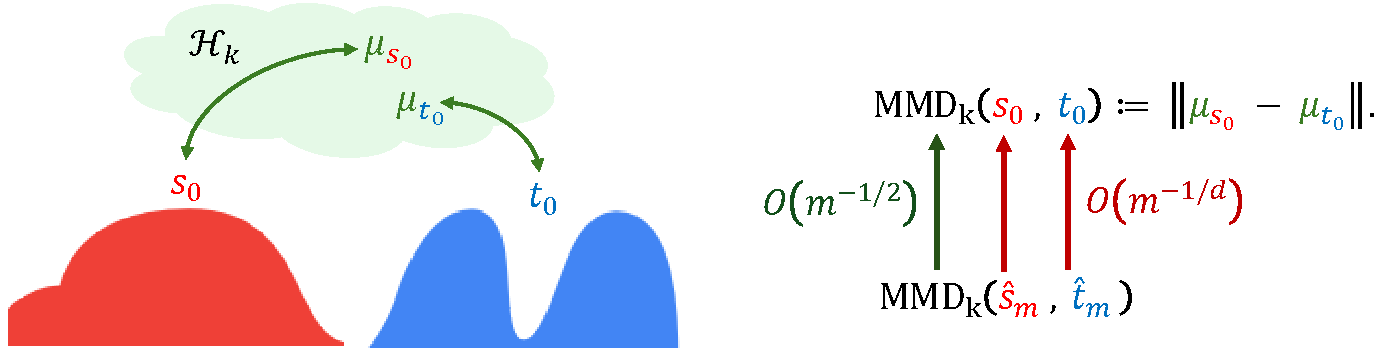
\includegraphics[width=0.9\linewidth]{background/images/MMD.pdf}
    \caption[Illustration of the MMD metric.]{Illustration of the MMD metric, which is the norm of the difference between kernel mean embeddings of the distributions in the RKHS space, $\calH_k$, associated with a normalized characteristic kernel $k$. The underlying data dimensionality is $d$, which adversarially affects the rate at which the empirical measures converge to true measures in terms of Wasserstein.}
    \label{fig:MMD}
\end{figure}
\resumetoc
\subsection{Computational Aspects}\label{bg:kernel-comp}
Unlike the variants of the OT problem, the MMD metric can be computed in closed-form using evaluations of the kernel $k$. $$\MMD^2(s_0, t_0) \equiv \mathbb{E}_{X\sim s_0, X'\sim s_0}[k(X, X')] + \mathbb{E}_{Y\sim t_0,Y'\sim t_0}[k(Y, Y')] -2\mathbb{E}_{X\sim s_0, Y\sim t_0}[k(X, Y)].$$
With the given empirical measures $\hat{s}_m=\sum_{i=1}^m(\mathbf{s}_m)_i\delta_{x_{1i}}$ and $\hat{t}_n=\sum_{j=1}^n(\mathbf{t}_n)_j\delta_{x_{2j}}$, we have
$\MMD^2(\hat{s}_m, \hat{t}_m) = \mathbf{s}_m^\top \bG_{11}\mathbf{s}_m+\mathbf{t}_n^\top \bG_{22}\mathbf{t}_n - 2\mathbf{s}_m^\top \bG_{12}\mathbf{t}_n$, where $\bG_{11}\in \R^{m\times m}$ is the Gram matrix over the given samples $\{x_{11}, \ldots, x_{1m}\}$ from $s_0$, $\bG_{22}\in \R^{n\times n}$ is the Gram matrix over the given samples $\{x_{21}, \ldots, x_{2m}\}$ from $t_0$ and $\bG_{12}\in \R^{m\times n}$ is the matrix with each entry as kernel function’s evaluation between the corresponding sample from $s_0$ and $t_0$, i.e. $(\bG_{12})_{ij} = k(x_{1i}, x_{2j})\ \forall i\in [m], j\in [n]$. Given the Gram matrices, the computation of MMD can be done in $O(m^2)$.
The memory needed to store the Gram matrices can be reduced using popular methods like Nystr$\ddot{\textup{o}}$m approximation.
% To reduce the memory requirements for storing the Gram matrices $\bG\in \R^{m\times m}$, a widely used approach is that of Nystr$\ddot{\textup{o}}$m approximation to randomly sample $l<m$ columns from $\bG$ and compute the kernel evaluations between the original samples and these $l$ representative samples.

\subsection{Statistical Aspects}\label{bg:kernel-stats}
For $s\in \calR^+(\calX)$, let the Kernel Mean Embedding (KME) be denoted as $\mu_s$, and the KME of the empirical measure $\hat{s}_m$ be denoted as $(\hat{\mu}_s)_m$. The following result from \citet[Theorem (3.4)]{Muandet_2017} shares the results on statistical convergence.
\begin{theorem}
    Let $k:\calX\times \calX\mapsto \R$ be a positive definite kernel with $\sup_{x\in \calX}k(x, x)<C_k<\infty$. Then, for any $\delta\in (0, 1)$, with probability at least $1-\delta$,
    $$\|(\hat{\mu}_s)_m- \mu_s\|_k\leq \frac{1}{\sqrt{m}}\left(\sqrt{C_k}+\sqrt{2C_k\log\frac{1}{\delta}} \right).$$
\end{theorem}
We note that for a normalized kernel, $\sup_{x\in \calX}k(x, x)=1$, and the RHS in the above inequality is independent of data dimensionality.
This result says that with $\hat{s}_m$ denoting the empirical measure for the true measure $s_0$, $\MMD(\hat{s}_m, s_0) \stackrel{(w.h.p.)}{\leq} O(m^{-1/2})$.


Using the triangle inequality, $\MMD(s_0, t_0)-\MMD(\hat{s}_m, \hat{t}_m)\leq \MMD(s_0, \hat{s}_m) + \MMD(t_0, \hat{t}_m) \implies \left|\MMD(s_0, t_0)-\MMD(\hat{s}_m, \hat{t}_m)\right| \stackrel{(w.h.p.)}{\leq} O(m^{-1/2})$. This is pictorially shown in Fig.~\ref{fig:MMD}.
\newline
\newline
\textit{This concludes our main discussion on the background materials for this thesis. Preliminaries specific to our contributions in the forthcoming chapters are separately discussed in those chapters.}